\section{Konklusion}
Arbejdet med opgaven har givet indsigt, dels i brugen af stored procedures, og dels i brugen af functions.

Til at teste om vores system har virket, er der blevet brugt en MS SQL localDB. Siden er databasen bevet deployed til den eksterne i4dab.ase.au.dk server. 

En af de udfordringer vi stødte på undervejs var at få vores ConnectionString til at virke. På skærmudsnittende nedenfor (figur~\ref{fig:measurement_remote} og \ref{fig:sensor_remote}) kan database indholdet af hhv. Measurements og Sensors på den eksterne DAB server ses.
% hvordan programmet er testet

% billede hvor man kan se a\ref{fig:measurement_remote}t lortet virker, goes here
\begin{figure}
\centering
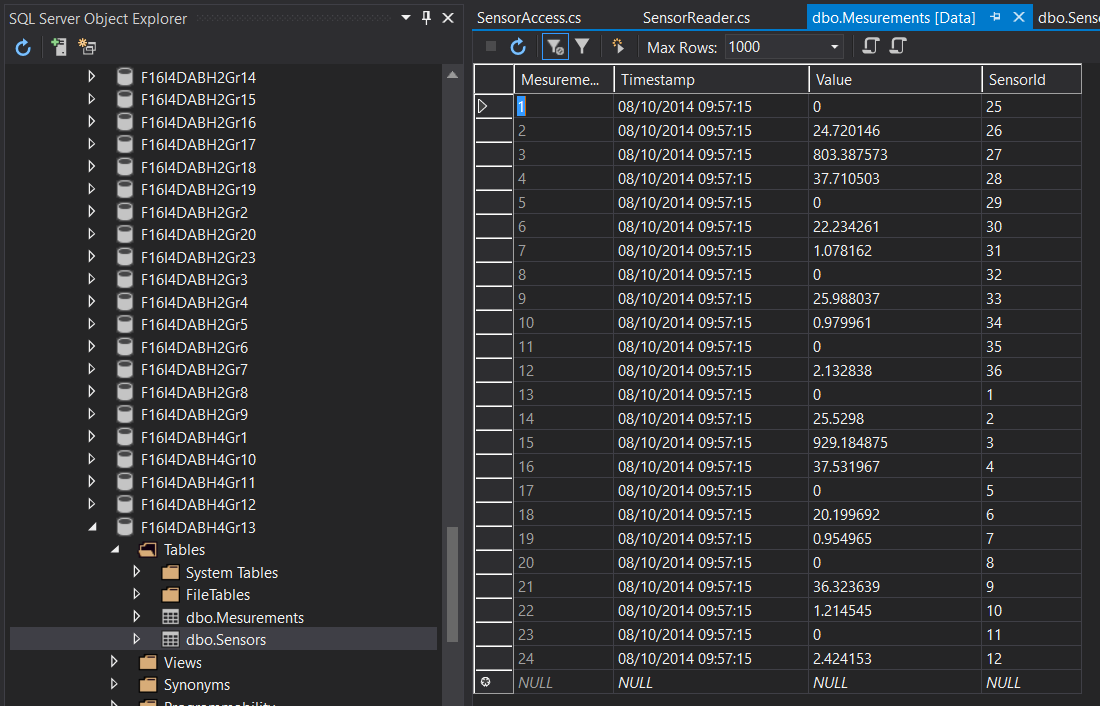
\includegraphics[width=\linewidth]{figs/measurement_remote}
\caption{Skærmudsnit af dataindhold på ekstern server - Measurements}
\label{fig:measurement_remote}
\end{figure}

\begin{figure}
	\centering
	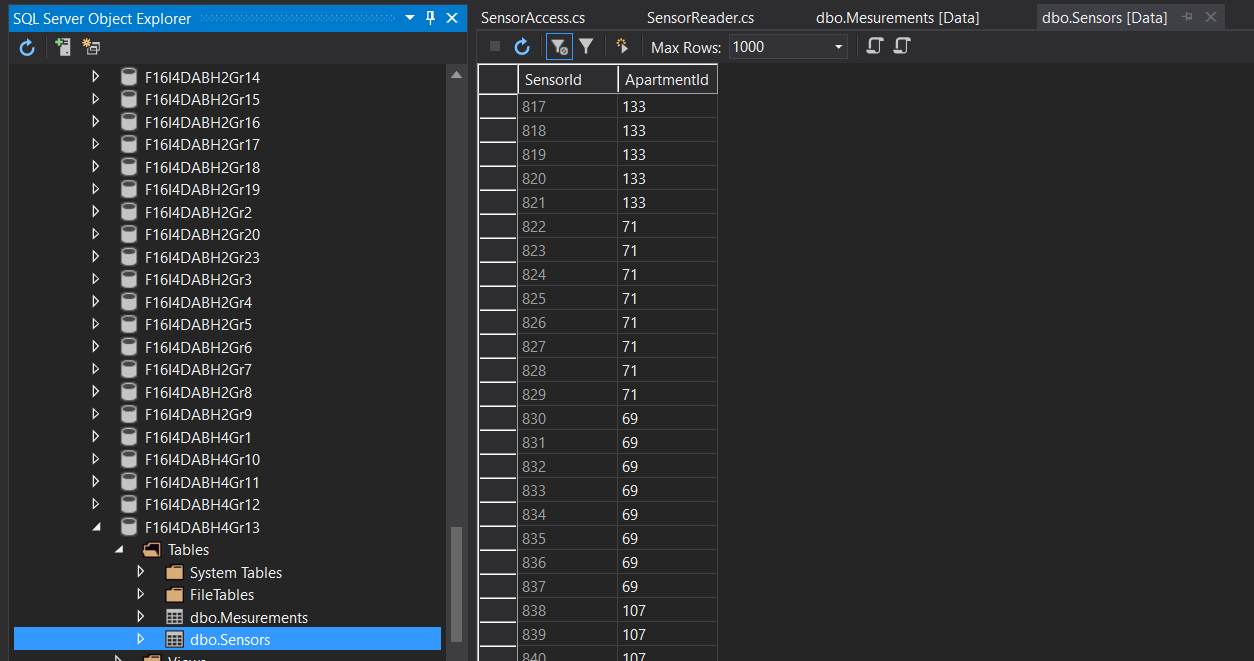
\includegraphics[width=\linewidth]{figs/sensor_remote}
	\caption{Skærmudsnit af dataindhold på ekstern server - Sensor}
	\label{fig:sensor_remote}
\end{figure}